% Offizielle Beispieldatei für beamer-Vorlage aus tubslatex Version 0.3beta2
\documentclass[fleqn,11pt,aspectratio=43]{beamer}

%\usepackage{etex}
%\reserveinsert{28}

\usepackage[ngerman]{babel}
\usepackage[autostyle=true,german=quotes]{csquotes}
\usepackage[utf8x]{inputenc}
\usepackage{graphicx}
\usepackage{listings}
\PassOptionsToPackage{svgnames}{xcolor}
\usepackage{color}
\usepackage{pxfonts}

%\usepackage{DejaVuSansMono}
\usetheme[%
  %cmyk,%<cmyk/rgbprint>,          Auswahl des Farbmodells
  orange,%<blue/orange/green/violet> Auswahl des Sekundärfarbklangs
  %dark,%<light,medium>        Auswahl der Helligkeit
  %colorhead,%    Farbig hinterlegte Kopfleiste
  %colorfoot,%    Farbig hinterlegt Fußleiste auf Titelseite
  colorblocks,%   Blöcke Farbig hinterlegen
  %nopagenum,%    Keine Seitennumer in Fußzeile
  %nodate,%       Kein Datum in Fußleiste
  %tocinheader,%   Inhaltsverzeichnis in Kopfleiste
  %tinytocinheader,% kleines Kopfleisten-Inhaltsverzeichnis
  %widetoc,%      breites Kopfleisten-Inhaltsverzeichnis
  %narrowtoc,%    schmales Kopfleisten-Inhaltsverzeichnis
  %nosubsectionsinheader,%  Keine subsections im Kopfleisten-Inhaltsverzeichnis
  %nologoinfoot,% Kein Logo im Fußbereich darstellen
  ]{tubs}

% Titelgrafik, automatisch beschnitten, Weitere Optionen: <scaled/cropx/cropy>
%\titlegraphic[scaled]{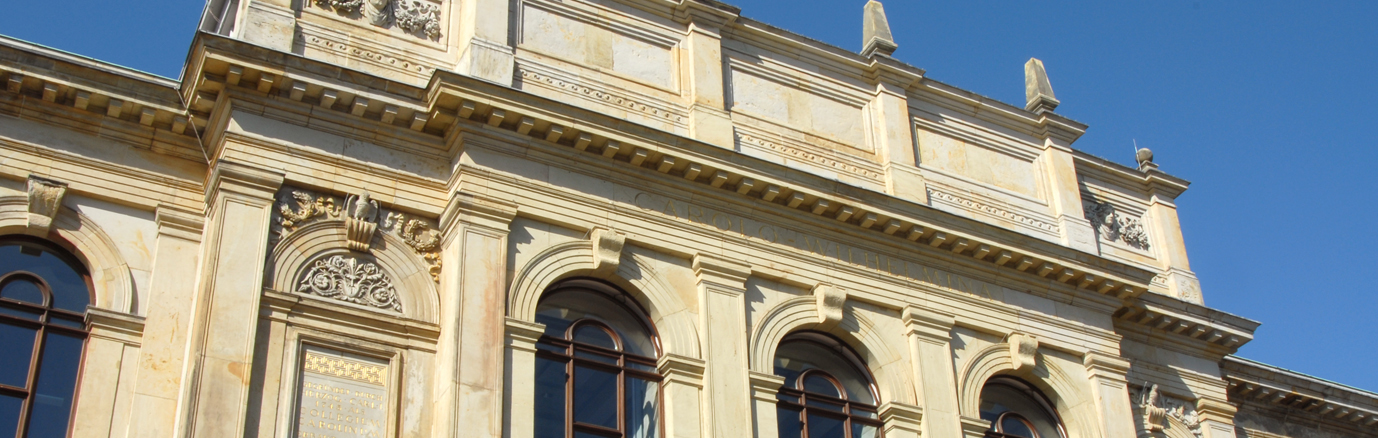
\includegraphics{img/titlepicture.jpg}}
\titlegraphic[cropy]{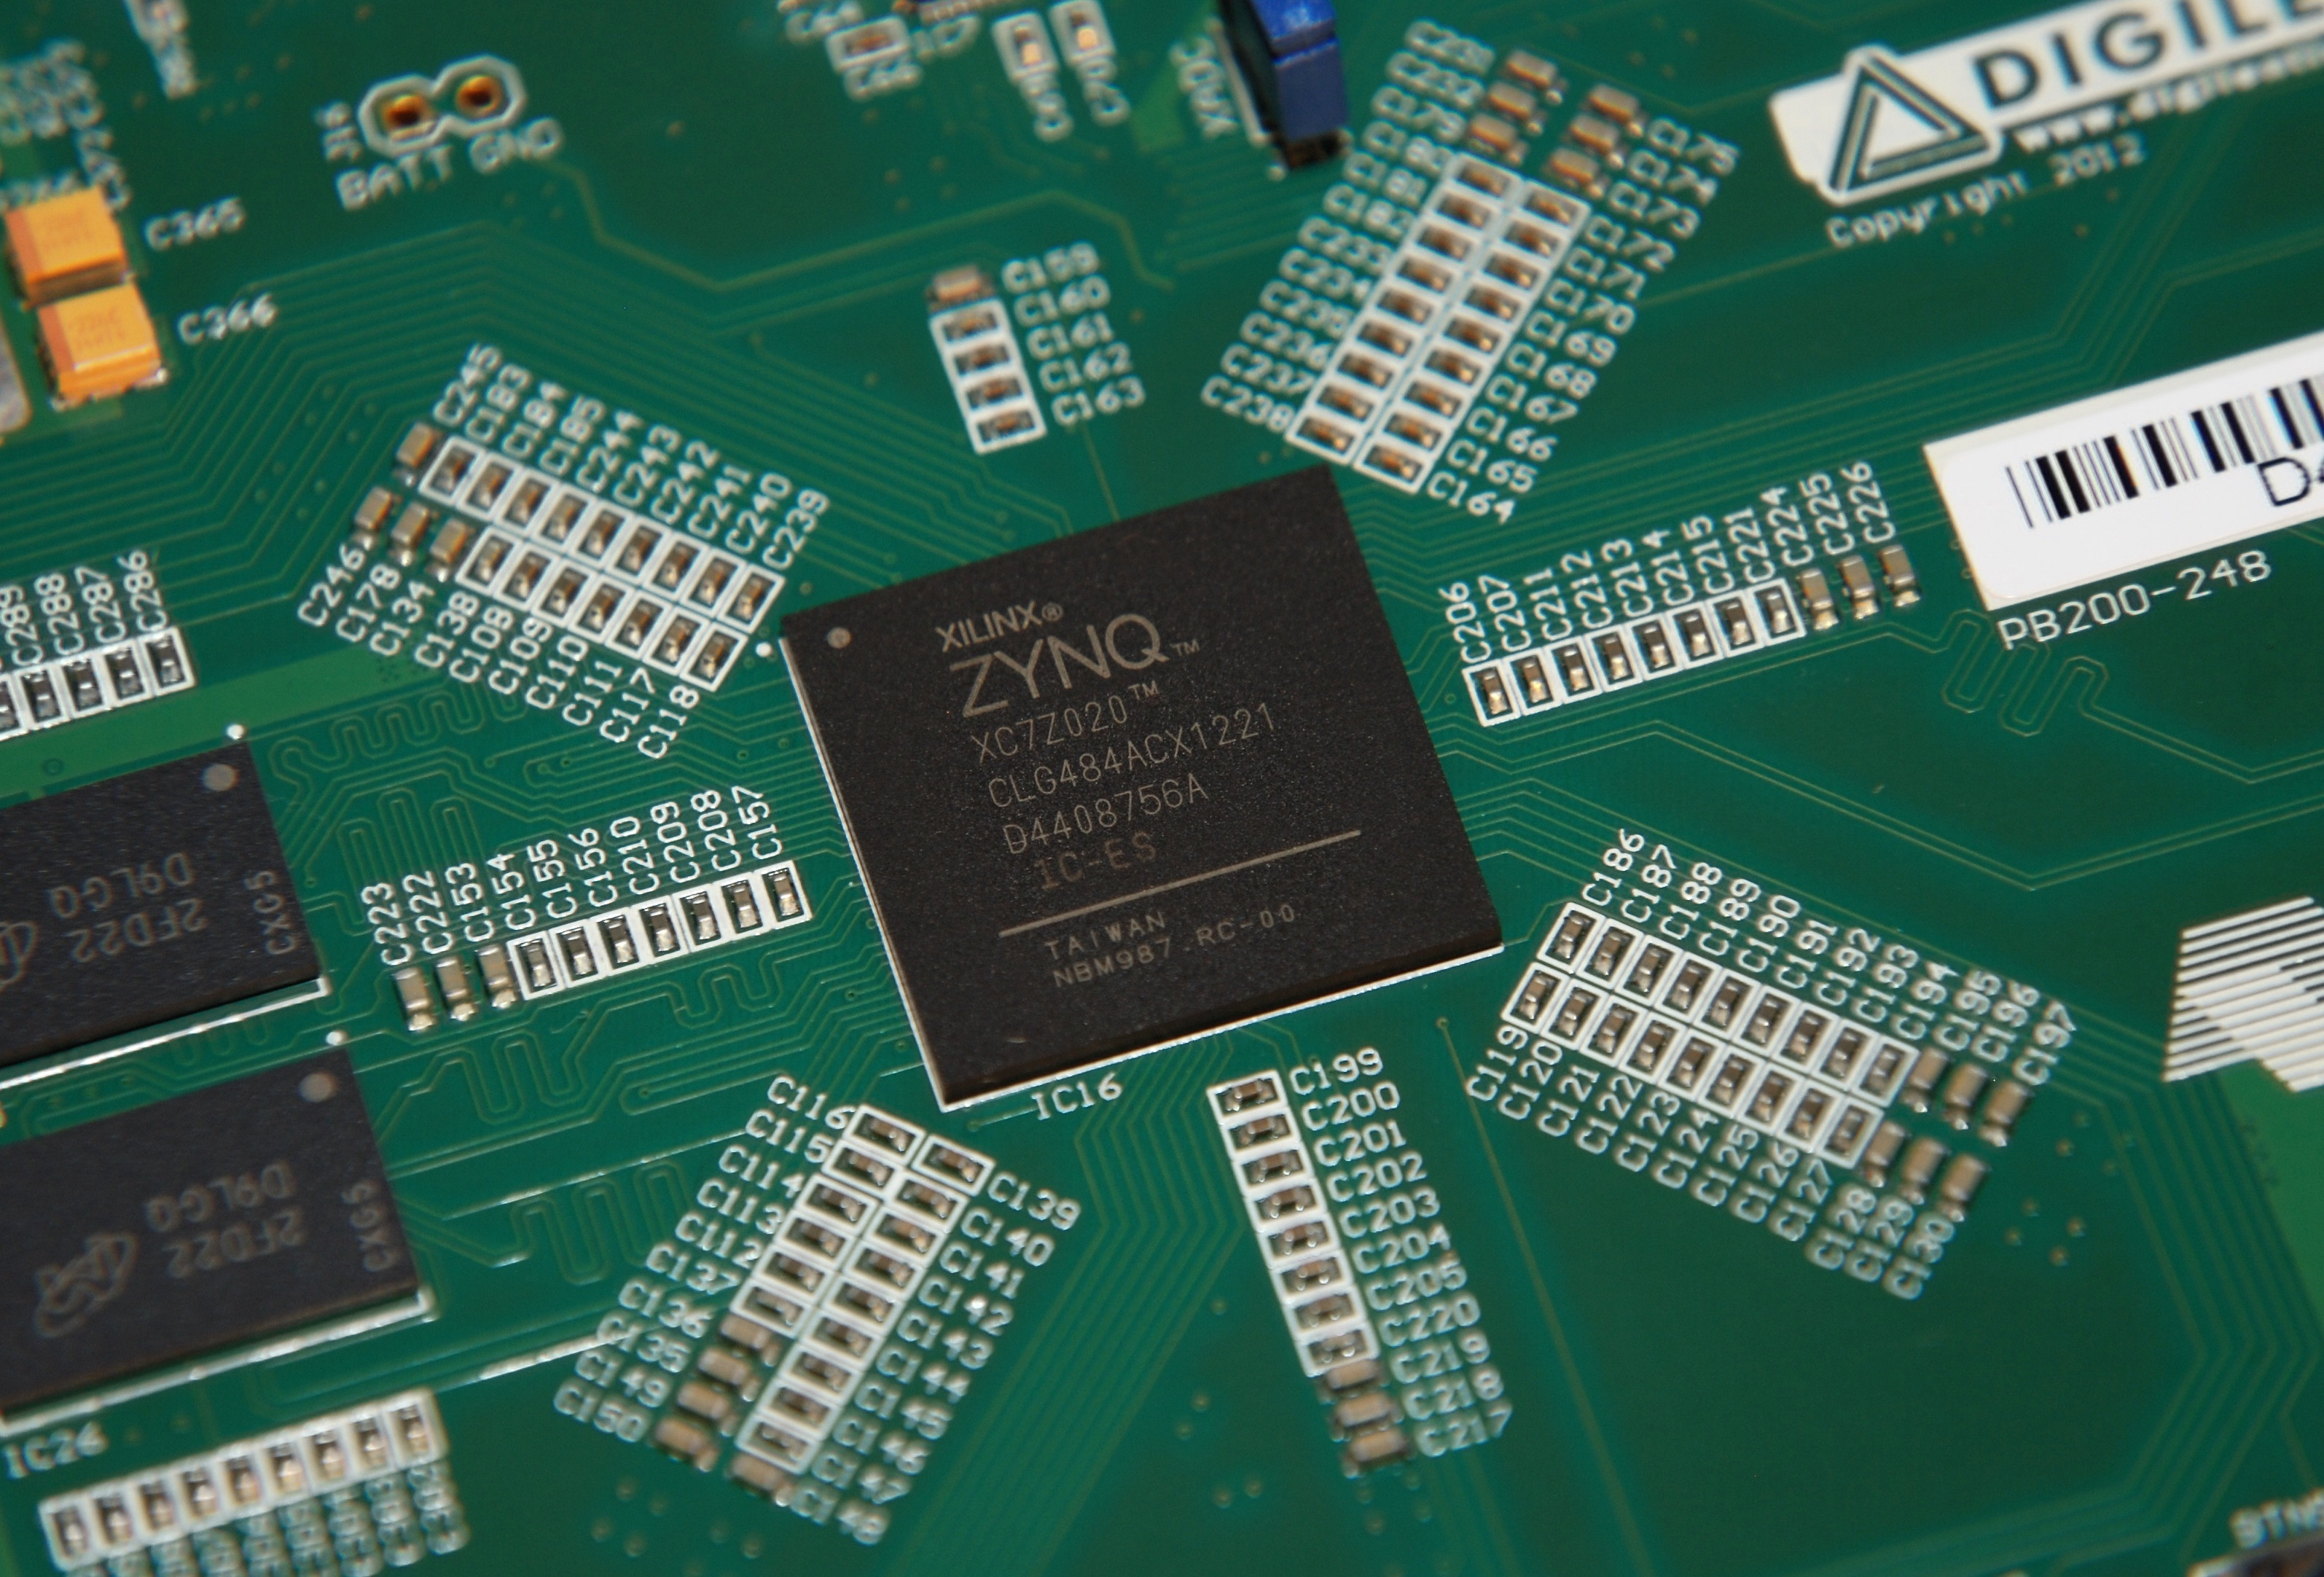
\includegraphics{img/zynq.jpg}}

% Logo, dass auf Titelseiten oben rechts und auf Inthaltsseiten unten rechts
% dargestellt wird. Es wird jeweils automatisch skliert
\logo{
\includegraphics{img/logo_mit_text.pdf}}

% settings for source code highlighting
\lstset{ %
  backgroundcolor=\color{white},         % choose the background color
  %basicstyle=\ttfamily\footnotesize,     % size of fonts used for the code
  basicstyle=\ttfamily\footnotesize,     % size of fonts used for the code
  breaklines=true,                       % automatic line breaking only at whitespace
  captionpos=b,                          % sets the caption-position to bottom
  commentstyle=\color{tuGreenDark80},    % comment style
  escapeinside={\%*}{*)},                % if you want to add LaTeX within your code
  keywordstyle=\color{tuBlueMedium100}\bfseries, % keyword style
  stringstyle=\color{tuVioletMedium},    % string literal style
}

%\AtBeginSection[]{
%  \begin{frame}[noframenumbering] 
%  		\scriptsize
%  		\frametitle{Überblick}  
%  		\tableofcontents[currentsection, subsectionstyle=show]
%  \end{frame}
%}

%\AtBeginSubsection[]{
%  \begin{frame}[noframenumbering]
%    	\scriptsize 
%  		\frametitle{\insertsectionhead - \insertsubsectionhead} 
%  		\tableofcontents[ 
%  			currentsubsection, 
%  		    sectionstyle=show/hide, 
%  		   	subsectionstyle=show/shaded/hide] 
%  \end{frame}
%}

\usepackage{tikz}
\usetikzlibrary{decorations.markings}

\pgfdeclarelayer{edgelayer}
\pgfdeclarelayer{nodelayer}
\pgfsetlayers{edgelayer,nodelayer,main}

\tikzstyle{none}=[inner sep=0pt]
\definecolor{hexcolor0x0074ff}{rgb}{0.000,0.455,1.000}
\definecolor{hexcolor0xff2615}{rgb}{1.000,0.149,0.082}

\definecolor{myblack}{rgb}{0.000,0.000,0.000}
\definecolor{mywhite}{rgb}{1.000,1.000,1.000}

\tikzstyle{setA}=[circle,fill=hexcolor0x0074ff,draw=myblack]
\tikzstyle{setB}=[circle,fill=hexcolor0xff2615,draw=myblack]
\tikzstyle{node}=[circle,fill=mywhite,draw=myblack,scale=.1]

\usepackage{enumitem}
\setitemize{label=\usebeamerfont*{itemize item}%
  \usebeamercolor[fg]{itemize item}
  \usebeamertemplate{itemize item}}

\usepackage{eqlist}
\let\description=\eqlist
\let\enddescription=\endeqlist
\let\eqlistlabel\descriptionlabel

\DeclareMathOperator{\dist}{dist}
\DeclareMathOperator{\RSS}{RSS}

% Titelseite
\title{Seminar Technische Informatik}
\subtitle{Top 10 algorithms in data mining}
\author{Stephan Mielke}
\date{22.01.2015}

\begin{document}

\begin{frame}[plain, noframenumbering]
\titlepage
\end{frame}

%\begin{frame}{Inhalt}
%\tableofcontents
%\end{frame}

\section*{Motivation~}

\begin{frame}[plain]{\insertsectionhead - Der Weltraum unendliche Weiten \dots}

\begin{figure}
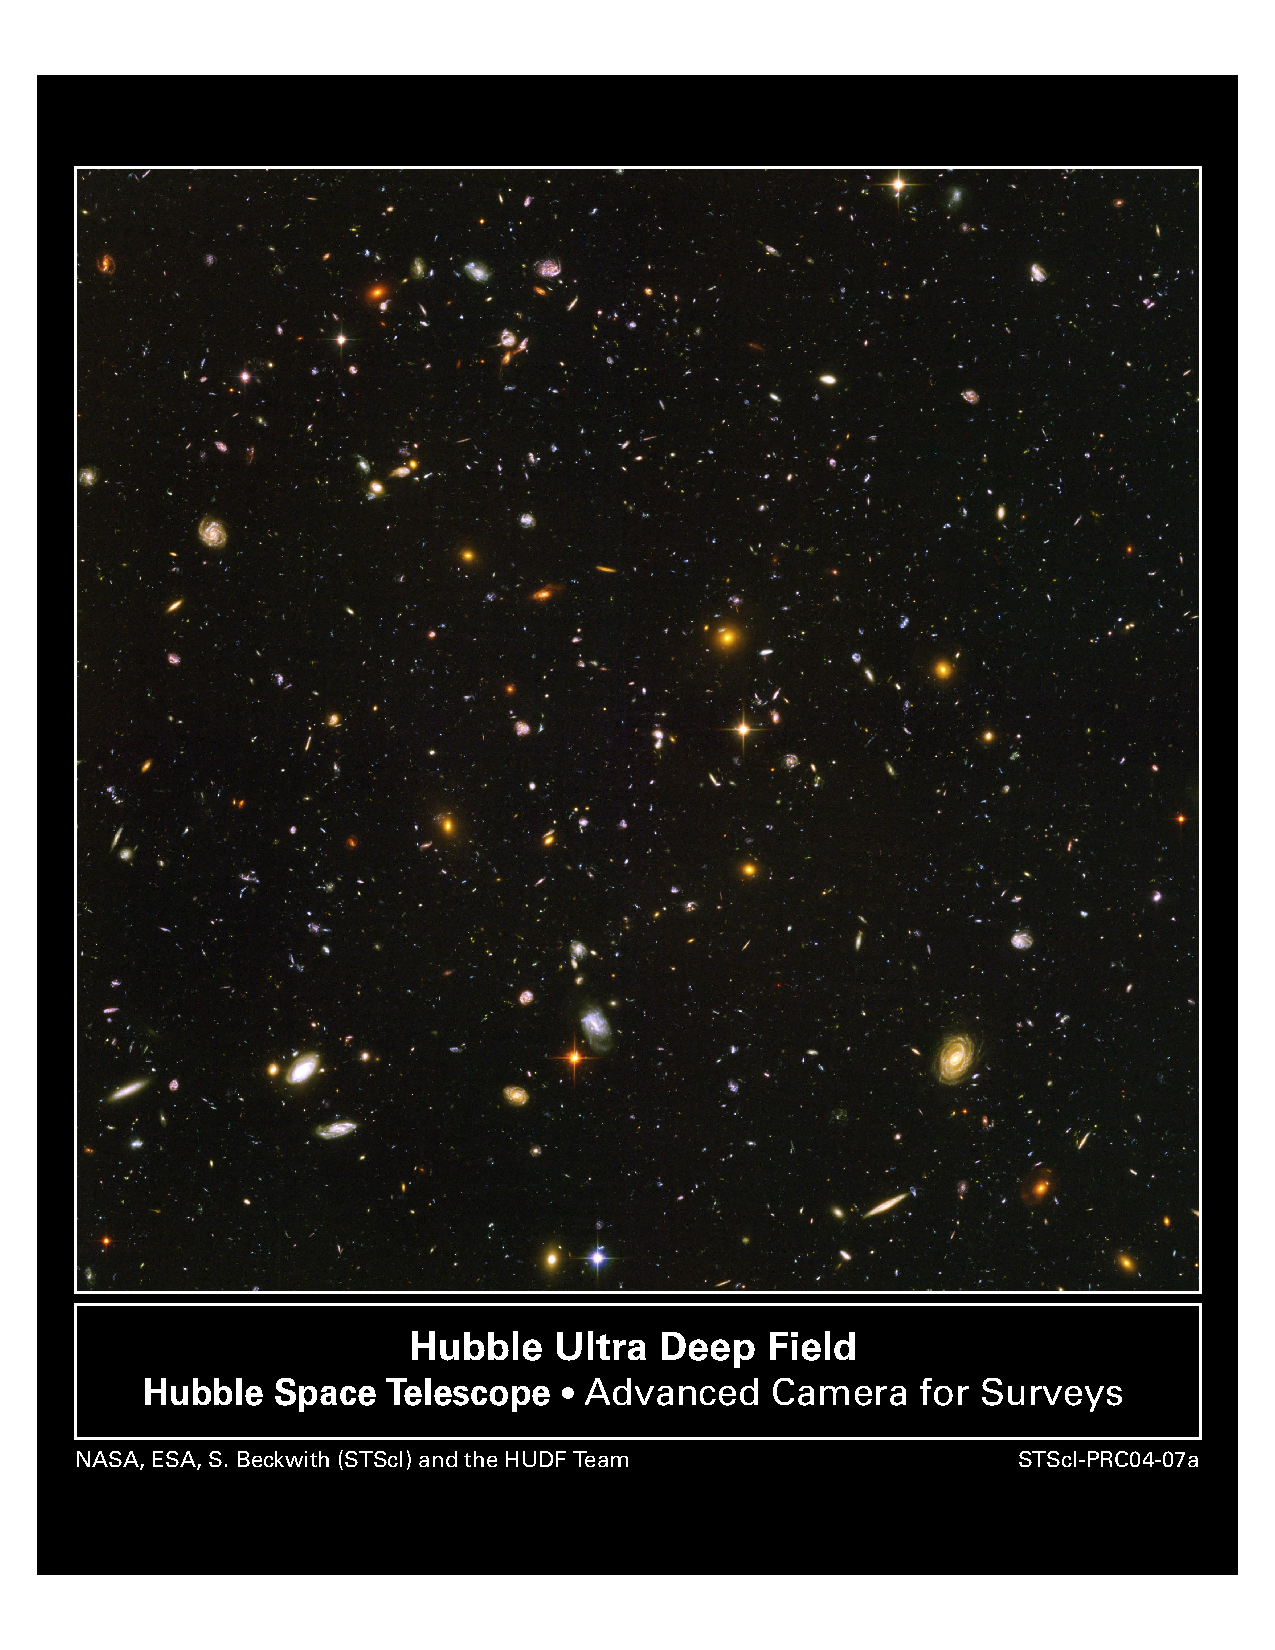
\includegraphics[scale=0.6,trim={40 400 40 80},clip]{hs-2004-07-a-pdf}
\caption{Hubble Ultra Deep Field \cite{HUDF}}
\label{fig:hs-2004-07-a-pdf}
\end{figure}
\end{frame}

\begin{frame}{\insertsectionhead - Einsatz von DM in der Astronomie}
\begin{itemize}
\item Klassifizierung von Sternen mit $k$-nearest neighbor ($k$-nn)
\item Manuelle Klassifizierung unmöglich  \cite{ester2000knowledge}
\item Pro Bild mehre $10000$ Objekte
\item Kepler z.B. hat 13.2m Objekte erkannt
\item Benutzung von Klassifizierungsalgorithmen aus DM
\end{itemize}
\begin{columns}[onlytextwidth]
    \column{0.4\textwidth}
    	\vspace{-5.2em}
		\begin{itemize}
		\item Je Objekt 9 Attribute (8 Isophotenformen, Leuchtkraft)
		\item Ausgabewert \enquote{stellary}
		\begin{itemize}
		\item $0.0 - 0.1$ Galaxie
		\item $0.9 - 1.0$ Stern
		\end{itemize}
		\end{itemize}
    \column{0.6\textwidth}
	    \begin{table}
	    \begin{tabular}{l|l}
	    Name & Erkennung\\ \hline
	    Random Forest & $82,89\%$ \\
	    Decision Tree & $80,68\%$ \\
	    Artificial Neural Network & $75.82\%$ \\
	    Support Vector Machines & $37,82\%$ \\
	    \end{tabular}
	    \caption{Erkennungsraten der Algorithmen Stern / Galaxie \cite{o2009star}}
	    \end{table}
\end{columns}
\end{frame}

\section{Data Mining~}

\begin{frame}{\insertsectionhead - Einleitung \cite{ester2000knowledge}}
\small
\vspace{-1em}
\begin{itemize} % beide folien zusammen
\setlength{\itemsep}{-3pt}
%\item Gehört zum Gebiet des Knowledge Discovery in Databases (KDD)
\item Idee: \textbf{Wissen} durch \textbf{Daten}
\item Einsatz in der Forschung, Vermarktung, Medizin, (Wetter)-Vorhersagen, 
Betrugsaufklärung usw.
\end{itemize}
\vspace{-1em}
\begin{block}{Definition nach Fayyad \cite{fayyad1996data}}
Knowledge Discovery in Databases describes the non-trivial process of 
identifying valid, novel, potentially useful, and ultimately understandable 
patterns in data.
\begin{figure}
\vspace{-2.7em} \hspace{-1.5em}
\includegraphics[page=5,scale=0.67,trim={51 500 65 86},clip]{dm_fayyad.pdf}
%\caption{KDD nach Fayyad \cite{fayyad1996data}}
\label{fig:fayyad1996data}
\end{figure}
\vspace{-3.5em}
\end{block}
\end{frame}

%\begin{frame}{\insertsectionhead - Einordnung}
%
%\end{frame}

%\begin{frame}{\insertsectionhead - Algorithmen Kategorien}
%\begin{block}{}
%\centering
%\alert<1>{There are known knowns,} [...]\\
%\alert<2>{There are known unknowns}, [...]\\
%\alert<3>{There are also unknown unknowns}\footnote{Donald H. Rumsfeld, US 
%Secretary of 
%Defense at a US Department of Defense news briefing, 12 February 
%2002} \cite{AstronomicalDM}
%\end{block}
%
%\begin{alertblock}{}
%\centering
%\only<1>{Klassifikation}
%\only<2>{Regression}
%\only<3>{Clustering}
%\only<4>{Assoziation}
%\end{alertblock}
%\end{frame}


\subsection{Top 10 algorithms in data mining~}
\begin{frame}{\insertsectionhead - \insertsubsectionhead \cite{wu2008top}}
\begin{itemize}
\item Anlass: IEEE International Conference on Data Mining
\item Datum: Dezember 2006
\item Erstellung: Jeder ACM KDD Innovation Award oder IEEE ICDM Research 
Contributions Award Preisträger nominierte 10 Algorithmen
\item Nur Nominierte mit $\geq$ 50 Referenzierungen in \emph{Google Scholar}
\item 
{\small\url{http://www.cs.uvm.edu/~icdm/algorithms/CandidateList.shtml}}
\item Per Abstimmung finden der Top 10
\item Das Paper: Top 10 algorithms in data mining  \cite{wu2008top}
\end{itemize}
\end{frame}

\begin{frame}{\insertsectionhead - \insertsubsectionhead \cite{wu2008top}}
% zuordnungen zusammen fassen, vorstellen rot usw
\small
\vspace{-0.6em}
\begin{block}{\vspace{-0.2em}Clustering\vspace{-0.2em}}
\vspace{-1.5em}
\begin{columns}[onlytextwidth]
    \column{0.5\textwidth}
		\begin{enumerate}[label=\bfseries\arabic*.]
		\setlength{\itemsep}{-5pt}
		\item \textbf{C4.5 und ähnliche}
		\item \textbf{\textcolor{red}{k-means}}
		\item \textcolor{red}{Suport Vector Machines}
		\item Apriori
		\item \textbf{EM Algorithm}
		\end{enumerate}
    \column{0.5\textwidth}
	    \begin{enumerate}[label=\bfseries\arabic*.]
	    \setlength{\itemsep}{-5pt}
	    \setcounter{enumi}{5}
	    \item PageRank
	    \item AdaBoost
	    \item k-nearest neighbor
	    \item Naive Bayes
	    \item \textbf{CART}
	    \end{enumerate}
\end{columns}
\vspace{-0.3em}
\end{block}
\pause
\vspace{-0.4em}
\begin{block}{\vspace{-0.2em}Classification\vspace{-0.2em}}
\vspace{-1.5em}
\begin{columns}[onlytextwidth]
    \column{0.5\textwidth}
		\begin{enumerate}[label=\bfseries\arabic*.]
		\setlength{\itemsep}{-5pt}
		\item C4.5 und ähnliche
		\item \textcolor{red}{k-means}
		\item \textbf{\textcolor{red}{Suport Vector Machines}}
		\item Apriori
		\item EM Algorithm
		\end{enumerate}
    \column{0.5\textwidth}
	    \begin{enumerate}[label=\bfseries\arabic*.]
	    \setlength{\itemsep}{-5pt}
	    \setcounter{enumi}{5}
	    \item PageRank
	    \item \textbf{AdaBoost}
	    \item \textbf{k-nearest neighbor}
	    \item \textbf{Naive Bayes}
	    \item CART
	    \end{enumerate}
\end{columns}
\vspace{-0.3em}
\end{block}
\pause
\vspace{-0.4em}
\begin{block}{\vspace{-0.2em}Assoziation\vspace{-0.2em}}
\vspace{-1.5em}
\begin{columns}[onlytextwidth]
    \column{0.5\textwidth}
		\begin{enumerate}[label=\bfseries\arabic*.]
		\setlength{\itemsep}{-5pt}
		\item C4.5 und ähnliche
		\item \textcolor{red}{k-means}
		\item \textcolor{red}{Suport Vector Machines}
		\item \textbf{Apriori}
		\item EM Algorithm
		\end{enumerate}
    \column{0.5\textwidth}
	    \begin{enumerate}[label=\bfseries\arabic*.]
	    \setlength{\itemsep}{-5pt}
	    \setcounter{enumi}{5}
	    \item PageRank
	    \item AdaBoost
	    \item k-nearest neighbor
	    \item Naive Bayes
	    \item CART
	    \end{enumerate}
\end{columns}
\vspace{-0.3em}
\end{block}
\end{frame}

%\begin{frame}{\insertsectionhead - \insertsubsectionhead}
%
%\end{frame}

\subsection{Clustering~}

\begin{frame}{\insertsectionhead - \insertsubsectionhead - Einleitung \cite{ester2000knowledge}}
\begin{itemize}
\item Einordnung von Objekten in unbekannten Klassen
\item Finden der Funktion die Objekte gruppiert
%\item Cluster haben unterschiedliche Formen, sind verschachtelt usw.
\item Ähnlichkeit von Objekten durch eine Distanzfunktion ermitteln
\end{itemize}
\end{frame}

\begin{frame}{\insertsectionhead - \insertsubsectionhead - Cluster \cite{dwh}}
\begin{itemize}
\item Formen: sehr unterschiedlich
\item Flach oder Hierarchisch
\item Anzahl von Clustern:
\begin{itemize}
\item Festgelegte Anzahl von $k$-Clustern
\item Anzahl hängt von der Qualitätsgüte der Cluster ab
\end{itemize} 
\item Qualitätsgüte: nicht zu klein oder groß
\item Hard oder Soft - Clustering
\item Keine großen \enquote{Lücken} zwischen den Daten
\item Cluster durch Heuristiken sonst zu großer Aufwand
\end{itemize}
\end{frame}

\begin{frame}{\insertsectionhead - \insertsubsectionhead - Distanzfunktion \cite{ester2000knowledge}}
\begin{itemize} % ToDo folien mergen
\item Menge von Objekten $O = \{o_1, o_2, \ldots, o_n\}$
\item Jedes Objekt $x$ hat $x_i$ Attribute
\item Es muss gelten 1.-3., für Metrik 4.:
\begin{align}
\dist(o_1, o_2) &= d \in R^{n\geq 0}\\
\dist(o_1, o_2) &= 0 \mbox{ genau dann wenn } o_1 = o_2\\
\dist(o_1, o_2) &= \dist(o_2, o_1) \mbox{ (Symmetrie)}\\
\dist(o_1, o_3) &\leq \dist(o_1, o_2) + \dist(o_2, o_3)
\end{align}
\item Attributarten und jeweilige beispielhafte Distanzfunktionen:
\begin{itemize}  
\item Nummerisch $\dist(x,y) = \sqrt{(x_1 - y_1)^2 + \ldots + (x_n - y_n)^2}$
\item Kategorisch ~$\dist(x,y) = \sum\limits_{i=1}^{n}\delta(x_i, y_i)$,~~~~~ $\delta(x_i, y_i) = \begin{cases}
0  ,x_i = y_i\\
1  ,x_i \neq y_i
\end{cases} $
\end{itemize}
%\item Manchmal auch Ähnlichkeitsfunktion genannt $\Rightarrow$ Interpretation anders herum.
\end{itemize}
\end{frame}

%\begin{frame}[fragile]{\insertsectionhead - \insertsubsectionhead - Distanzfunktion \cite{ester2000knowledge}}
%\small
%\vspace{-0.5em}
%\begin{itemize}
%\item Datensätze $x = (x_1, \ldots, x_n)$ mit nummerischen Attributen $x_i$
%\only<1>{\begin{description}
%\item[Euklidische-Distanz:] $\dist(x,y) = \sqrt{(x_1 - y_1)^2 + \ldots + (x_n - y_n)^2}$
%\item[Manhattan-Distanz:] $\dist(x,y) = |x_1 - y_1| + \ldots + |x_n - y_n|$
%\item[Maximum-Metrik:] $\dist(x,y) = \max\big(|x_1 - y_1| + \ldots + |x_n - y_n|\big)$
%\item[Alg. $L_p$-Metrik:] $\dist(x,y) = \sqrt[p]{\sum\limits_{i=1}^{d}{(x_i-y_i)^p}}$
%\end{description}}
%\item Datensätze $x = (x_1, \ldots, x_n)$ mit kategorischen Attributen $x_i$
%\only<1>{\begin{itemize}
%%\item Summe der Unterschiede
%\item $\dist(x,y) = \sum\limits_{i=1}^{a}\delta(x_i, y_i)$
%\item $\delta(x_i, y_i) \ \ \ = \begin{cases}
%0 \mbox{ wenn } (x_i = y_i)\\
%1 \mbox{ wenn } (x_i \neq y_i)
%\end{cases} $
%\end{itemize}}
%\item Endliche Mengen $x = \{x_1, \ldots, x_n\}$\\
%\only<1>{
%\begin{description}
%\item[Anteil verschiedener:] $\dist(x,y) = \frac{|x\cup y| - |x \cap y|}{|x \cup y|}$
%\end{description}
%}
%\end{itemize}
%\end{frame}

\begin{frame}{\insertsectionhead - \insertsubsectionhead - Beispiel \cite{ester2000knowledge}}
\begin{itemize} % mergen
\item Clustering von Web-Sessions zur Bestimmung von Benutzergruppen
\item Datenquelle: Logfile eines Webservers
\item Eintrag: IP, User-ID, Timestamp, URL, \ldots
\item Einträge werden nach Session gruppiert, nach einem Zeitfenster
\item Session: IP, User-ID, Liste von URLs
\item URLs werden geclustert, z.B.: Distanzfunktion für endliche Mengen
\item Wissen:
\begin{itemize}
\item Benutzergruppen / Benutzerprofilen, für Marketingstrategien 
\item URLs sind durch Interessen verbunden, Optimierung für Zugriffsgewohnheiten 
\end{itemize}
\item Ein Sozialmediabutton kann auch die nötigen Informationen liefern.
\end{itemize}
\end{frame}


\subsubsection{k-means~}\label{kmeans}

\begin{frame}{\insertsectionhead - \insertsubsectionhead - $k$-means \cite{dwh}}
\begin{itemize}
\item Hartes Flaches Clustering
\item Bekannte Anzahl von $k$ Clustern
\item Daten als Vektoren
\item Idee: Minimiert den Abstand vom Clusterschwerpunkt zu den Daten
\item Cluster ist Definiert als:
\begin{itemize}
\item $A = \{d_l, \ldots, d_m\}$, $A$ ist ein Cluster und $d_i$ Element 
\item $\mu(A) = \frac{l}{m}\sum\limits_{i=l}^{m}{d_i}$ ist Schwerpunkt
\end{itemize}
\item Qualität: gut wenn $\RSS(\ldots)$ minimal ist
\begin{description}
\item[Cluster:] $\RSS\,(A) = \sum\limits_{i=l}^{m}\big\|d_i - \mu(A)\big\|^2$
\item[Gesamt:] $\RSS\,(A_l, \ldots, A_k) = \sum\limits_{j=l}^{k}\,\RSS\,(A_j)$
\end{description}
\end{itemize}
\end{frame}

\begin{frame}{\insertsectionhead - \insertsubsectionhead - $k$-means \cite{dwh}}
Der $k$-means Algorithmus (Lloyd's Algorithmus)
\begin{enumerate}[label=\bfseries\arabic*.]
\item Selektiere zufällig $k$ Schwerpunkte als Startwert
\item Erstelle $k$ leere Cluster
\item Weise jedem Cluser einen Schwerpunkt zu
\item Weise jedem Datenvektor den den Cluster mit dem nächstem Schwerpunkt zu
\item Berechne den Schwerpunkt jedes Clusters neu
\item Teste ob die Qualität des Clusterings ausreicht, sonst gehe zu 2.
\end{enumerate}
\end{frame}

\begin{frame}{\insertsectionhead - \insertsubsectionhead - $k$-means}
\begin{figure}
\scalebox{1.1}{\tikzstyle{none}=[inner sep=0pt]
\definecolor{hexcolor0x0074ff}{rgb}{0.000,0.455,1.000}
\definecolor{hexcolor0xff2615}{rgb}{1.000,0.149,0.082}

\definecolor{myblack}{rgb}{0.000,0.000,0.000}
\definecolor{mywhite}{rgb}{1.000,1.000,1.000}

\tikzstyle{sp}=[circle,fill=myblack,draw=myblack, scale=1]
\tikzstyle{setA}=[circle,fill=hexcolor0x0074ff,draw=myblack]
\tikzstyle{setB}=[circle,fill=hexcolor0xff2615,draw=myblack]
\tikzstyle{setC}=[circle,fill=mywhite,draw=myblack]
\tikzstyle{node}=[circle,fill=mywhite,draw=myblack,scale=.1]


\begin{tikzpicture}
	%\begin{pgfonlayer}{nodelayer}
		\node [style=setC] (0) at (-1.75, 1.75) {};
		\node [style=setC] (1) at (-3, 0.5) {};
		\node [style=setC] (2) at (0,2) {};
		\node [style=setC] (3) at (-1.25, 0.75) {};
		\node [style=setC] (4) at (-2.25, 1) {};
		\node [style=setC] (5) at (-3.25, 1.75) {};
		\node [style=setC] (6) at (-1.75, 2.75) {};
		\node [style=setC] (7) at (-1, 1.5) {};
		\node [style=setC] (8) at (2.25, 1.5) {};
		\node [style=setC] (9) at (1.25, 0.75) {};
		\node [style=setC] (10) at (2.75, -0.25) {};
		\node [style=setC] (11) at (0,-0.5) {};
		\node [style=setC] (12) at (3.25, 1) {};
		\node [style=setC] (13) at (2, 0.5) {};
		\node [style=setC] (14) at (2.5, -1.5) {};
		\node [style=setC] (15) at (-1,-1.5) {};
		\node [style=setC] (16) at (1.25, -1.75) {};
		\node [style=setC] (17) at (1.75, -0.25) {};
		\node [style=setC] (18) at (-2.25, -0.25) {};
		\node [style=setC] (19) at (1.75, 1) {};

\node [sp] at (-1,-0.5) {};
\node [sp] at (1,1.5) {};
\end{tikzpicture}}
\caption{Ersten 3 Phasen, $k = 2$}
\end{figure}
\end{frame}

\begin{frame}{\insertsectionhead - \insertsubsectionhead - $k$-means}
\begin{figure}
\scalebox{1.1}{\tikzstyle{none}=[inner sep=0pt]
\definecolor{hexcolor0x0074ff}{rgb}{0.000,0.455,1.000}
\definecolor{hexcolor0xff2615}{rgb}{1.000,0.149,0.082}

\definecolor{myblack}{rgb}{0.000,0.000,0.000}
\definecolor{mywhite}{rgb}{1.000,1.000,1.000}

\tikzstyle{sp}=[circle,fill=myblack,draw=myblack, scale=1]
\tikzstyle{setA}=[circle,fill=hexcolor0x0074ff,draw=myblack]
\tikzstyle{setB}=[circle,fill=hexcolor0xff2615,draw=myblack]
\tikzstyle{setC}=[circle,fill=mywhite,draw=myblack]
\tikzstyle{node}=[circle,fill=mywhite,draw=myblack,scale=.1]


\begin{tikzpicture}
		\node [style=setA] (0) at (-1.75, 1.75) {};
		\node [style=setB] (1) at (-3, 0.5) {};
		\node [style=setA] (2) at (0,2) {};
		\node [style=setB] (3) at (-1.25, 0.75) {};
		\node [style=setB] (4) at (-2.25, 1) {};
		\node [style=setB] (5) at (-3.25, 1.75) {};
		\node [style=setA] (6) at (-1.75, 2.75) {};
		\node [style=setA] (7) at (-1, 1.5) {};
		\node [style=setA] (8) at (2.25, 1.5) {};
		\node [style=setA] (9) at (1.25, 0.75) {};
		\node [style=setA] (10) at (2.75, -0.25) {};
		\node [style=setB] (11) at (0,-0.5) {};
		\node [style=setA] (12) at (3.25, 1) {};
		\node [style=setA] (13) at (2, 0.5) {};
		\node [style=setB] (14) at (2.5, -1.5) {};
		\node [style=setB] (15) at (-1,-1.5) {};
		\node [style=setB] (16) at (1.25, -1.75) {};
		\node [style=setA] (17) at (1.75, -0.25) {};
		\node [style=setB] (18) at (-2.25, -0.25) {};
		\node [style=setA] (19) at (1.75, 1) {};

\node [sp] (v1) at (-1,-0.5) {};
\node [sp] (v2) at (1,1.5) {};
\draw  (3) edge (v1);
\draw  (11) edge (v1);
\draw  (15) edge (v1);
\draw  (18) edge (v1);
\draw  (4) edge (v1);
\draw  (1) edge (v1);
\draw  (5) edge (v1);
\draw  (16) edge (v1);
\draw  (14) edge (v1);
\draw  (6) edge (v2);
\draw  (0) edge (v2);
\draw  (7) edge (v2);
\draw  (2) edge (v2);
\draw  (9) edge (v2);
\draw  (19) edge (v2);
\draw  (8) edge (v2);
\draw  (12) edge (v2);
\draw  (13) edge (v2);
\draw  (17) edge (v2);
\draw  (10) edge (v2);
\end{tikzpicture}}
\caption{Phase 4, Zuordnung nur beispielhaft}
\end{figure}
\end{frame}

\begin{frame}{\insertsectionhead - \insertsubsectionhead - $k$-means}
\begin{figure}
\scalebox{1.1}{\tikzstyle{none}=[inner sep=0pt]
\definecolor{hexcolor0x0074ff}{rgb}{0.000,0.455,1.000}
\definecolor{hexcolor0xff2615}{rgb}{1.000,0.149,0.082}

\definecolor{myblack}{rgb}{0.000,0.000,0.000}
\definecolor{mywhite}{rgb}{1.000,1.000,1.000}

\tikzstyle{sp}=[circle,fill=myblack,draw=myblack, scale=1]
\tikzstyle{setA}=[circle,fill=hexcolor0x0074ff,draw=myblack]
\tikzstyle{setB}=[circle,fill=hexcolor0xff2615,draw=myblack]
\tikzstyle{setC}=[circle,fill=mywhite,draw=myblack]
\tikzstyle{node}=[circle,fill=mywhite,draw=myblack,scale=.1]


\begin{tikzpicture}
		\node [style=setA] (0) at (-1.75, 1.75) {};
		\node [style=setB] (1) at (-3, 0.5) {};
		\node [style=setA] (2) at (0,2) {};
		\node [style=setB] (3) at (-1.25, 0.75) {};
		\node [style=setB] (4) at (-2.25, 1) {};
		\node [style=setB] (5) at (-3.25, 1.75) {};
		\node [style=setA] (6) at (-1.75, 2.75) {};
		\node [style=setA] (7) at (-1, 1.5) {};
		\node [style=setA] (8) at (2.25, 1.5) {};
		\node [style=setA] (9) at (1.25, 0.75) {};
		\node [style=setA] (10) at (2.75, -0.25) {};
		\node [style=setB] (11) at (0,-0.5) {};
		\node [style=setA] (12) at (3.25, 1) {};
		\node [style=setA] (13) at (2, 0.5) {};
		\node [style=setB] (14) at (2.5, -1.5) {};
		\node [style=setB] (15) at (-1,-1.5) {};
		\node [style=setB] (16) at (1.25, -1.75) {};
		\node [style=setA] (17) at (1.75, -0.25) {};
		\node [style=setB] (18) at (-2.25, -0.25) {};
		\node [style=setA] (19) at (1.75, 1) {};

\node [none] (v2) at (-1,-0.5) {};
\node [none] (v3) at (1,1.5) {};

\node [sp] (v1) at (-1.5,0) {};
\node [sp] (v4) at (1.5,1) {};
\draw  (v2) edge (v1);
\draw  (v3) edge (v4);
\end{tikzpicture}}
\caption{Phase 5, Schwerpunkte sind nur beispielhaft}
\end{figure}
\end{frame}

\begin{frame}{\insertsectionhead - \insertsubsectionhead - $k$-means}
\begin{figure}
\scalebox{1.1}{\tikzstyle{none}=[inner sep=0pt]
\definecolor{hexcolor0x0074ff}{rgb}{0.000,0.455,1.000}
\definecolor{hexcolor0xff2615}{rgb}{1.000,0.149,0.082}

\definecolor{myblack}{rgb}{0.000,0.000,0.000}
\definecolor{mywhite}{rgb}{1.000,1.000,1.000}

\tikzstyle{sp}=[circle,fill=myblack,draw=myblack, scale=1]
\tikzstyle{setA}=[circle,fill=hexcolor0x0074ff,draw=myblack]
\tikzstyle{setB}=[circle,fill=hexcolor0xff2615,draw=myblack]
\tikzstyle{setC}=[circle,fill=mywhite,draw=myblack]
\tikzstyle{node}=[circle,fill=mywhite,draw=myblack,scale=.1]

\begin{tikzpicture}
		\node [style=setB] (0) at (-1.75, 1.75) {};
		\node [style=setB] (1) at (-3, 0.5) {};
		\node [style=setA] (2) at (0,2) {};
		\node [style=setB] (3) at (-1.25, 0.75) {};
		\node [style=setB] (4) at (-2.25, 1) {};
		\node [style=setB] (5) at (-3.25, 1.75) {};
		\node [style=setB] (6) at (-1.75, 2.75) {};
		\node [style=setB] (7) at (-1, 1.5) {};
		\node [style=setA] (8) at (2.25, 1.5) {};
		\node [style=setA] (9) at (1.25, 0.75) {};
		\node [style=setA] (10) at (2.75, -0.25) {};
		\node [style=setB] (11) at (0,-0.5) {};
		\node [style=setA] (12) at (3.25, 1) {};
		\node [style=setA] (13) at (2, 0.5) {};
		\node [style=setA] (14) at (2.5, -1.5) {};
		\node [style=setB] (15) at (-1,-1.5) {};
		\node [style=setA] (16) at (1.25, -1.75) {};
		\node [style=setA] (17) at (1.75, -0.25) {};
		\node [style=setB] (18) at (-2.25, -0.25) {};
		\node [style=setA] (19) at (1.75, 1) {};
		
\node [sp] (v1) at (-1.5,0) {};
\node [sp] (v4) at (1.5,1) {};

\draw  (v1) edge (3);
\draw  (7) edge (v1);
\draw  (0) edge (v1);
\draw  (4) edge (v1);
\draw  (1) edge (v1);
\draw  (5) edge (v1);
\draw  (6) edge (v1);
\draw  (18) edge (v1);
\draw  (15) edge (v1);
\draw  (11) edge (v1);
\draw  (2) edge (v4);
\draw  (9) edge (v4);
\draw  (19) edge (v4);
\draw  (8) edge (v4);
\draw  (12) edge (v4);
\draw  (13) edge (v4);
\draw  (10) edge (v4);
\draw  (17) edge (v4);
\draw  (16) edge (v4);
\draw  (14) edge (v4);
\end{tikzpicture}}
\caption{Phase 6 und noch mal von Phase 2 an}
\end{figure}
\end{frame}

\subsection{Classification~}

\begin{frame}{\insertsectionhead - \insertsubsectionhead - Einleitung \cite{ester2000knowledge}}
\begin{itemize}
\item Einordnung von Objekten in bekannten Klassen
\item Trainingsdaten für Klassen $\Rightarrow$ Klassen bekannt
\item Finden der Funktion die Objekte möglichst genau zuordnet
\item Teilaufgaben:
\begin{itemize}
\item Zuordnung zu einer Klasse
\item Generierung von Wissen 
\end{itemize}
\end{itemize}
\end{frame}

\begin{frame}{\insertsectionhead - \insertsubsectionhead - Training \cite{ester2000knowledge}}
\begin{itemize}
\item Menge von Objekten $O = \{o_1, o_2, \ldots, o_n\}$
\item Klasse $c_i \in C = \{c_1, c_2, \ldots, c_n\}$ für jedes Objekt ist bekannt
\item Jedes Objekt hat $A_i$ Klassifizierung-Attribute
\item Attributarten:
\begin{itemize}
\item Kategorische Attribute
\item Nummerische Attribute
\end{itemize}
\end{itemize}
\end{frame}

\begin{frame}[fragile]{\insertsectionhead - \insertsubsectionhead - Beispiel \cite{ester2000knowledge}}
Trainingsdaten:
\begin{table}
\begin{tabular}{|p{2cm}|p{2cm}|p{2cm}|p{2cm}|}\hline
ID 	& Alter	& Autotyp	& Risikoklasse \\\hline \hline
1	& 23	& Familie	& Hoch\\
2	& 17	& Sport		& Hoch\\
3	& 43	& Sport		& Hoch\\
4	& 68	& Familie	& Niedrig\\
5	& 32	& LKW		& Niedrig \\\hline
\end{tabular}
\caption{Beispiele aus Knowledge discovery in databases: Techniken und Anwendungen \cite{ester2000knowledge}}
\end{table}
\pause
Das gesuchte Wissen
\begin{lstlisting}[language=Haskell]
if Alter > 50                    then Risikoklasse = Niedrig
if Alter <= 50 and Autotyp = LKW then Risikoklasse = Niedrig
                                 else Risikoklasse = Hoch
\end{lstlisting}
\end{frame}

\begin{frame}{\insertsectionhead - \insertsubsectionhead - Gesuchte Wissen \cite{ester2000knowledge}}
\begin{description}
\item[Formen:]
\begin{itemize}
\item Entscheidungsbaum % geordnet nach Informationsgewinn
\item Funktion % alles mögliche, 
\item Vektor im Koordinatensystem
\end{itemize}
\item[Anwendung:] Immer dann, wenn die Klassen bekannt sind
\begin{itemize}
\item Unterscheidung von Stern / Galaxie
\item Sterne Einordnen
\item Zuordnung von Risikogruppen
\item Medizinforschung
\item \dots
\end{itemize}
\end{description}
\end{frame}

\subsubsection{Support vector machines~}\label{svm}

\begin{frame}{\insertsectionhead - \insertsubsectionhead - SVM \cite{dwh}}
\begin{description}
\item[Annahmen:]
\begin{itemize}
\item Nur zwei Klassen
\item Jedes Objekt ist ein Vektor im Koordinatensystem
\end{itemize}
\item[Ziel:]  Hyperplane\footnote{Hyperebene} die den Raum teilt 
\item[Training:]
\begin{itemize}
\item Hyperplane mit maximalem Abstand zu allen Trainingsvektoren
\item Hyperplane Begrenzungsobjekte sind Supportvektoren
\end{itemize} 
\item[Differenzfunktion:] $\delta(o_1, o_2)$ ist ähnlich zum Clustering
\end{description}
\end{frame}

\begin{frame}{\insertsectionhead - \insertsubsectionhead - SVM}
%Bild bei der die richtige Teilung gesucht wird (F 55)
\begin{figure}
\scalebox{.7}{\tikzstyle{none}=[inner sep=0pt]
\definecolor{hexcolor0x0074ff}{rgb}{0.000,0.455,1.000}
\definecolor{hexcolor0xff2615}{rgb}{1.000,0.149,0.082}

\definecolor{myblack}{rgb}{0.000,0.000,0.000}
\definecolor{mywhite}{rgb}{1.000,1.000,1.000}

\tikzstyle{setA}=[circle,fill=hexcolor0x0074ff,draw=myblack]
\tikzstyle{setB}=[circle,fill=hexcolor0xff2615,draw=myblack]
\tikzstyle{node}=[circle,fill=mywhite,draw=myblack,scale=.1]


\begin{tikzpicture}
	%\begin{pgfonlayer}{nodelayer}
		\node [style=setA] (0) at (-1.75, 1.75) {};
		\node [style=setA] (1) at (-3, 0.5) {};
		\node [style=setA] (2) at (0,2) {};
		\node [style=setA] (3) at (-1.25, 0.75) {};
		\node [style=setA] (4) at (-2.25, 1) {};
		\node [style=setA] (5) at (-3.25, 1.75) {};
		\node [style=setA] (6) at (-1.75, 2.75) {};
		\node [style=setA] (7) at (-1, 1.5) {};
		\node [style=setB] (8) at (2.25, 1.5) {};
		\node [style=setB] (9) at (1.25, 0.75) {};
		\node [style=setB] (10) at (2.75, -0.25) {};
		\node [style=setB] (11) at (0,-0.5) {};
		\node [style=setB] (12) at (3.25, 1) {};
		\node [style=setB] (13) at (2, 0.5) {};
		\node [style=setB] (14) at (2.5, -1.5) {};
		\node [style=setB] (15) at (-1,-1.5) {};
		\node [style=setB] (16) at (1.25, -1.75) {};
		\node [style=setB] (17) at (1.75, -0.25) {};
		\node [style=setA] (18) at (-2.25, -0.25) {};
		\node [style=setB] (19) at (1.75, 1) {};
		\node [style=node] (20) at (1,3.5) {};
		\node [style=node] (21) at (-2,-3.5) {};
		\node [style=node] (22) at (-4.25, -1.5) {};
		\node [style=node] (23) at (4.25, 2.75) {};
		\node [style=node] (24) at (2.5, 3.5) {};
		\node [style=node] (25) at (-4.25, -3.5) {};
	%\end{pgfonlayer}
	%\begin{pgfonlayer}{edgelayer}
		\draw [ultra thick] (22) to (23);
		\draw [ultra thick] (20) to (21);
		\draw [ultra thick] (25) to (24);
	%\end{pgfonlayer}
\node [none] (v1) at (-3.5,3) {};
\node [none] (v2) at (-5,-3.5) {};
\node [none] (v3) at (5,4) {};
\node [none] (v4) at (2,-3.5) {};
\draw [ultra thick] (v1) edge (v2);
\draw [ultra thick] (v3) edge (v4);
\end{tikzpicture}}
\caption{Gesucht: die richtige Hyperplane}
\end{figure}
\end{frame}

\begin{frame}{\insertsectionhead - \insertsubsectionhead - SVM}
\begin{figure}
\scalebox{.8}{\tikzstyle{none}=[inner sep=0pt]
\definecolor{hexcolor0x0074ff}{rgb}{0.000,0.455,1.000}
\definecolor{hexcolor0xff2615}{rgb}{1.000,0.149,0.082}

\definecolor{myblack}{rgb}{0.000,0.000,0.000}
\definecolor{mywhite}{rgb}{1.000,1.000,1.000}

\tikzstyle{setA}=[circle,fill=hexcolor0x0074ff,draw=myblack]
\tikzstyle{setB}=[circle,fill=hexcolor0xff2615,draw=myblack]
\tikzstyle{node}=[circle,fill=mywhite,draw=myblack,scale=.1]


\begin{tikzpicture}
	%\begin{pgfonlayer}{nodelayer}
		\node [style=setA] (0) at (-1.75, 1.75) {};
		\node [style=setA] (1) at (-3, 0.5) {};
		\node [style=setA] (2) at (0,2) {};
		\node [style=setA] (3) at (-1.25, 0.75) {};
		\node [style=setA] (4) at (-2.25, 1) {};
		\node [style=setA] (5) at (-3.25, 1.75) {};
		\node [style=setA] (6) at (-1.75, 2.75) {};
		\node [style=setA] (7) at (-1, 1.5) {};
		\node [style=setB] (8) at (2.25, 1.5) {};
		\node [style=setB] (9) at (1.25, 0.75) {};
		\node [style=setB] (10) at (2.75, -0.25) {};
		\node [style=setB] (11) at (0,-0.5) {};
		\node [style=setB] (12) at (3.25, 1) {};
		\node [style=setB] (13) at (2, 0.5) {};
		\node [style=setB] (14) at (2.5, -1.5) {};
		\node [style=setB] (15) at (-1,-1.5) {};
		\node [style=setB] (16) at (1.25, -1.75) {};
		\node [style=setB] (17) at (1.75, -0.25) {};
		\node [style=setA] (18) at (-2.25, -0.25) {};
		\node [style=setB] (19) at (1.75, 1) {};
		\node [style=node] (20) at (1.5, 3.5) {};
		\node [style=node] (21) at (-4.5,-3) {};
		\node [style=node] (22) at (3.5, 3.5) {};
		\node [style=node] (23) at (-2.5,-3) {};
		\node [style=node] (24) at (-3.5, -3) {};
		\node [style=node] (25) at (2.5, 3.5) {};
	%\end{pgfonlayer}
	%\begin{pgfonlayer}{edgelayer}
	\filldraw[thick,fill=green,fill opacity=0.4] (20.center) -- (21.center) -- (23.center) -- (22.center) -- cycle;

		%\draw (21) to (20);
		%\draw (23) to (22);
		\draw [ultra thick] (24) to (25);
	%\end{pgfonlayer}
\end{tikzpicture}}
\caption{Gefunden: die richtige Hyperplane}
\end{figure}
\end{frame}

\begin{frame}{\insertsectionhead - \insertsubsectionhead - SVM}
\begin{figure}
\scalebox{.8}{\tikzstyle{none}=[inner sep=0pt]
\definecolor{hexcolor0x0074ff}{rgb}{0.000,0.455,1.000}
\definecolor{hexcolor0xff2615}{rgb}{1.000,0.149,0.082}

\definecolor{myblack}{rgb}{0.000,0.000,0.000}
\definecolor{mywhite}{rgb}{1.000,1.000,1.000}

\tikzstyle{setA}=[circle,fill=hexcolor0x0074ff,draw=myblack]
\tikzstyle{setB}=[circle,fill=hexcolor0xff2615,draw=myblack]
\tikzstyle{setc}=[circle,fill=mywhite,draw=myblack]
\tikzstyle{node}=[circle,fill=mywhite,draw=myblack,scale=.1]


\begin{tikzpicture}
	%\begin{pgfonlayer}{nodelayer}
		\node [style=setA] (0) at (-1.75, 1.75) {};
		\node [style=setA] (1) at (-3, 0.5) {};
		\node [style=setA] (2) at (0,2) {};
		\node [style=setA] (3) at (-1.25, 0.75) {};
		\node [style=setA] (4) at (-2.25, 1) {};
		\node [style=setA] (5) at (-3.25, 1.75) {};
		\node [style=setA] (6) at (-1.75, 2.75) {};
		\node [style=setA] (7) at (-1, 1.5) {};
		\node [style=setB] (8) at (2.25, 1.5) {};
		\node [style=setB] (9) at (1.25, 0.75) {};
		\node [style=setB] (10) at (2.75, -0.25) {};
		\node [style=setB] (11) at (0,-0.5) {};
		\node [style=setB] (12) at (3.25, 1) {};
		\node [style=setB] (13) at (2, 0.5) {};
		\node [style=setB] (14) at (2.5, -1.5) {};
		\node [style=setB] (15) at (-1,-1.5) {};
		\node [style=setB] (16) at (1.25, -1.75) {};
		\node [style=setB] (17) at (1.75, -0.25) {};
		\node [style=setA] (18) at (-2.25, -0.25) {};
		\node [style=setB] (19) at (1.75, 1) {};
		\node [style=node] (20) at (1.5, 3.5) {};
		\node [style=node] (21) at (-4.5,-3) {};
		\node [style=node] (22) at (3.5, 3.5) {};
		\node [style=node] (23) at (-2.5,-3) {};
		\node [style=node] (24) at (-3.5, -3) {};
		\node [style=node] (25) at (2.5, 3.5) {};
	%\end{pgfonlayer}
	%\begin{pgfonlayer}{edgelayer}
	
	%\end{pgfonlayer}
\node [setc] at (0,0.5) {};
\node [setc] at (1,1.5) {};
\node [setc] at (2,2.5) {};
\node [setc] at (2.5,2) {};
\node [setc] at (2.5,1) {};
\node [setc] at (0.5,-0.5) {};
\node [setc] at (1.5,-1.5) {};
\node [setc] at (2.5,-1) {};
\node [setc] at (3,0.5) {};
\node [setc] at (1,-0.5) {};
\node [setc] at (1,0.5) {};
\node [setc] at (-1,-0.5) {};
\node [setc] at (0,-1) {};
\node [setc] at (-2,-2) {};
\node [setc] at (-1.5,-2) {};
\node [setc] at (0,-1.5) {};
\node [setc] at (1,-1) {};
\node [setc] at (0,1.5) {};
\node [setc] at (1,2.5) {};
\node [setc] at (0.5,3.5) {};
\node [setc] at (-1.5,0) {};
\node [setc] at (-0.5,0.5) {};
\node [setc] at (-2.5,-1) {};
\node [setc] at (-4,-0.5) {};
\node [setc] at (-4,-2) {};
\node [setc] at (-3,-1.5) {};
\node [setc] at (-3,-0.5) {};
\node [setc] at (-4,1) {};
\node [setc] at (-1,2.5) {};
\node [setc] at (0,2.5) {};
\node [setc] at (-0.5,3) {};
\node [setc] at (1.5,3) {};
\node [setc] at (2.5,3) {};
\node [setc] at (-0.5,1) {};
\node [setc] at (0.5,1) {};
\node [setc] at (-2,-1) {};
\node [setc] at (-1.5,-1) {};
\node [setc] at (-3.5,-2) {};
\node [setc] at (-2.5,-2.5) {};

\filldraw[thick,fill=green,fill opacity=0.4] (20.center) -- (21.center) -- (23.center) -- (22.center) -- cycle;

		%\draw (21) to (20);
		%\draw (23) to (22);
		\draw [ultra thick] (24) to (25);
\end{tikzpicture}}
\caption{Einordnung: mit der richtige Hyperplane}
\end{figure}
\end{frame}

\begin{frame}{\insertsectionhead - \insertsubsectionhead - SVM}
%Bild mit blöden Testdaten (keine richtige Teilung möglich) (F 62)
\begin{figure}
\scalebox{1.0}{\tikzstyle{none}=[inner sep=0pt]
\definecolor{hexcolor0x0074ff}{rgb}{0.000,0.455,1.000}
\definecolor{hexcolor0xff2615}{rgb}{1.000,0.149,0.082}

\definecolor{myblack}{rgb}{0.000,0.000,0.000}
\definecolor{mywhite}{rgb}{1.000,1.000,1.000}

\tikzstyle{setA}=[circle,fill=hexcolor0x0074ff,draw=myblack]
\tikzstyle{setB}=[circle,fill=hexcolor0xff2615,draw=myblack]
\tikzstyle{node}=[circle,fill=mywhite,draw=myblack,scale=.1]


\begin{tikzpicture}
	%\begin{pgfonlayer}{nodelayer}
		\node [style=setA] (0) at (-1.75, 1.75) {};
		\node [style=setA] (1) at (-3, 0.5) {};
		\node [style=setA] (2) at (0,2) {};
		\node [style=setA] (3) at (1,0) {};
		\node [style=setA] (4) at (-2.25, 1) {};
		\node [style=setA] (5) at (-3.25, 1.75) {};
		\node [style=setA] (6) at (-1.75, 2.75) {};
		\node [style=setA] (7) at (-1, 1.5) {};
		\node [style=setB] (8) at (2.25, 1.5) {};
		\node [style=setB] (9) at (1.25, 0.75) {};
		\node [style=setB] (10) at (2.75, -0.25) {};
		\node [style=setB] (11) at (-1,0.5) {};
		\node [style=setB] (12) at (3.25, 1) {};
		\node [style=setB] (13) at (2, 0.5) {};
		\node [style=setB] (14) at (2.5, -1.5) {};
		\node [style=setB] (15) at (-1,-1.5) {};
		\node [style=setB] (16) at (1.25, -1.75) {};
		\node [style=setB] (17) at (1.75, -0.25) {};
		\node [style=setA] (18) at (-2.25, -0.25) {};
		\node [style=setB] (19) at (1.75, 1) {};

\end{tikzpicture}}
\caption{Training: ungünstige Daten}
\end{figure}
\end{frame}

%\begin{frame}{\insertsectionhead - \insertsubsectionhead - SVM \cite{dwh}}
%Mehrere Klassen:
%\begin{itemize}
%\item One-versus-all
%\item One-versus-one
%\end{itemize}
%
%Overfitting
%\begin{itemize}
%\item Zu viele Trainingsdaten für eine Eigenschaft
%\item Lösungen
%\begin{itemize}
%\item Cross-validation
%\item Regularization
%\end{itemize} 
%\end{itemize}
%\end{frame}
%
%\begin{frame}{\insertsectionhead - \insertsubsectionhead - SVM}
%%Bild mit Overfitting (F 65)
%\begin{figure}
%\scalebox{1.1}{\tikzstyle{none}=[inner sep=0pt]
\definecolor{hexcolor0x0074ff}{rgb}{0.000,0.455,1.000}
\definecolor{hexcolor0xff2615}{rgb}{1.000,0.149,0.082}

\definecolor{myblack}{rgb}{0.000,0.000,0.000}
\definecolor{mywhite}{rgb}{1.000,1.000,1.000}

\tikzstyle{setA}=[circle,fill=hexcolor0x0074ff,draw=myblack]
\tikzstyle{setB}=[circle,fill=hexcolor0xff2615,draw=myblack]
\tikzstyle{node}=[circle,fill=mywhite,draw=myblack,scale=.1]


\begin{tikzpicture}
	%\begin{pgfonlayer}{nodelayer}
		\node [style=setA] (0) at (-1.75, 1.75) {};
		\node [style=setA] (1) at (-2.5,0.5) {};
		\node [style=setA] (2) at (0,2) {};
		\node [style=setA] (3) at (-1.25, 0.75) {};
		\node [style=setA] (4) at (-2.25, 1) {};
		\node [style=setA] (5) at (-1,0) {};
		\node [style=setA] (6) at (0.5,1.5) {};
		\node [style=setA] (7) at (-1, 1.5) {};
		\node [style=setB] (8) at (1,2) {};
		\node [style=setB] (9) at (0,1) {};
		\node [style=setB] (10) at (0,0.5) {};
		\node [style=setB] (11) at (0,-0.5) {};
		\node [style=setB] (12) at (1,2.5) {};
		\node [style=setB] (13) at (0.5,1) {};
		\node [style=setB] (14) at (-0.5,-0.5) {};
		\node [style=setB] (15) at (-1,-1.5) {};
		\node [style=setB] (16) at (-1.5,-0.5) {};
		\node [style=setB] (17) at (-1,0.5) {};
		\node [style=setA] (18) at (-2.25, -0.25) {};
		\node [style=setB] (19) at (1,1.5) {};
		\node [style=node] (22) at (-3,-1.5) {};
		\node [style=node] (23) at (2,3) {};
	%\end{pgfonlayer}
	%\begin{pgfonlayer}{edgelayer}
		\draw [ultra thick] (22) to (23);
	%\end{pgfonlayer}
\end{tikzpicture}}
%\caption{Overfitting: zu nahe}
%\end{figure}
%\end{frame}

%\subsection{Regression~}
%
%\begin{frame}{\insertsectionhead - \insertsubsectionhead - Einleitung \cite{fahrmeir2007regressionsanalyse}}
%
%\end{frame}

\subsection{Assoziation~}

% erst erklären

\begin{frame}{\insertsectionhead - \insertsubsectionhead - Einleitung \cite{ester2000knowledge}}

\begin{alertblock}{Jedem bekannt?}
\begin{quote}
Kunden, die diesen Artikel gekauft haben, kauften auch
\end{quote}
\end{alertblock}
\pause
\begin{description}
%\item[Synonym:] Warenkorbanalyse
\item[Gesucht:] Beziehungen (Regeln: $A \Rightarrow B$) zwischen Objekten
\item[Benötigt:] Tranaktionsdatenbank (Einkaufshistory)
%\item[Beispiel:] $\{\mbox{Eier}, \mbox{Mehl}\} \Rightarrow \{\mbox{Butter}\}$
\end{description}
\pause
\begin{columns}[onlytextwidth]
 \small
    \column{0.4\textwidth}
    \begin{table}
    	    \hspace{-2em}\begin{tabular}{c|l}
    	    ID & Itemset\\ \hline
    	    1 & Brot, Kaffee, Milch, Kuchen\\
    	    2 & Kaffee, Milch, Kuchen\\
    	    3 & Brot, Butter, Kaffee, Milch\\
    	    4 & Milch, Kuchen\\
    	    5 & Brot, Kuchen\\
    	    6 & Brot
    	    \end{tabular}
    	    %\caption{Erkennungsraten der Algorithmen Stern / Galaxie \cite{o2009star}}
    	    \end{table}
    	    
    \column{0.6\textwidth}
    \vspace{-1.5em}
	   \begin{description}
		   \item[Support:] \{Kaffee, Milch\} $= 50\%$
		   \item[Support:] \{Kaffee, Kuchen, Milch\} $\approx 33\%$
		   \item[Support:] \{Kaffee, Milch\} $\Rightarrow$ \{Kuchen\} \\ $\approx 33\%$
		   \item[Konfidenz:] \{Kaffee, Milch\} $\Rightarrow$ \{Kuchen\} \\= $\frac{33\%}{50\%} \approx 66\%$
	   \end{description}
\end{columns}
\end{frame}

\begin{frame}{\insertsectionhead - \insertsubsectionhead - Grundbegriffe \cite{ester2000knowledge}}
\begin{description}
%\item bla
\item[Items:] $I = \{i_1, \ldots, i_m\}$, ein Itemset $X \subseteq I$
\item[Transaktionsset:] $D = \{T_1, \ldots, T_n\}$, für $T_i$ gilt: $T_i \subseteq I$
\item[Support der Menge:] $\delta(X,D)$: Anteil (\%) aller $T_i$ für die gilt $X \subseteq T_i$
\item[Assoziationsregel:] $R_i = X \Rightarrow Y$ es gilt: $X, Y \subseteq I$ und $X \cap Y = \emptyset$ 
\item[Support der Regel:] $\delta(R_i, D) = \delta(X \cup Y, D)$: Anteil (\%)
\item[Konfidenz der Regel:] $\phi(R_i, D) = \delta(Y, \{T_i\;|\;\forall T_i \in D \wedge X \subseteq T_i\})$
\item[Idee:] Finden von Regeln die einen Support und Konfidenz von einer gewissen Schwelle besitzen
\end{description}
\end{frame}
		
%\subsubsection{Apriori}\label{apriori}

\section{Big Data~}

\begin{frame}{\insertsectionhead - Einleitung \cite{mayer2014big} \cite{wu2014data}}
\begin{itemize}
\item Himmelskartografie-Projekt Sloan Digital Sky Survey startete 2000\footnote{Teleskop mit 2,5m Spiegel am Apache Point Observatory -- New Mexico}
\item Sammelte in der ersten Wochen mehr Daten als die gesamte Astronomie davor\\ \vspace{1em}

\item Bis 2010 ca. 140 TB Daten gesammelt (ca. 35\% Abdeckung)\\
		Sterne	$260\;562\;744$ und Galaxien $208\;478\;448$ \cite{sdss3_scope:Online}
\item 2019 geplanter Nachfolger Large Synoptic Survey Telescope\footnote{Teleskop mit 8,4m Spiegel am El-Peñón-Gipfel des Cerro Pachón -- Chile} \\ \vspace{1em}
\item[$\Rightarrow$] \textbf{Erzeugt alle 5 Tage 140 TB an Daten!}
\end{itemize}
\end{frame}

\begin{frame}{\insertsectionhead - Einleitung \cite{mayer2014big} \cite{wu2014data}}
\begin{itemize}
\item \enquote{Datenberge} wachsen immer weiter an
\begin{itemize}
\item Geschätzt 2007 an die $300$ Exabyte\footnote{1 Exabyte = $1\;000\;000$ TB} Daten 
\item Geschätzt 2013 an die $1200$ Exabyte Daten\footnote{in CDs: 5 Stapel zum Mond}
\end{itemize}
\item Verarbeitung riesiger Datenmengen zur Gewinnung von Wahrscheinlichkeiten
zu genaueren Vorhersagen
\begin{itemize}
\item Das eine E-Mail Spam ist
\item Das \enquote{dei} bei der Autokorrektur \enquote{die} heißt
\item Bewegungen von Menschen, ob dies eine Gefahr für selbstlenkende Fahrzeuge sind
\end{itemize}
\item Die Erkenntnis ist nicht das \textbf{WARUM} sondern das \textbf{WAS} 
\item \enquote{Was wir an
Genauigkeit auf der Mikroebene verlieren, gewinnen wir an Erkenntnis
auf der Makroebene.} \cite{mayer2014big}
\end{itemize}
\end{frame}

\begin{frame}{\insertsectionhead - HACE Theorem \cite{wu2014data}}
\begin{quote}
Big Data starts with large-volume, \underline{\textbf{H}}eterogeneous, 
\underline{\textbf{A}}utonomous sources with distributed and decentralized control, 
and seeks to explore \underline{\textbf{C}}omplex and \underline{\textbf{E}}volving relationships 
among data.
\end{quote} %\cite{wu2014data}
\begin{description}\setlength{\itemsep}{15pt}
\item[{\parbox[t]{4cm}{Huge Heterogeneous Data:}}] {\parbox[t]{6.3cm}{Viele unterschiedliche Repräsentationen der \enquote{Datenhaufen}}}
\item[{\parbox[t]{4cm}{Autonomous Sources:}}] {\parbox[t]{6.3cm}{Wahllose Generierung von Daten ohne zentrale Steuerung}}
\item[{\parbox[t]{4cm}{Complex and Evolving Relationships:}}] {\parbox[t]{6.3cm}{Verflechtung der Daten untereinander wird immer komplexer und nimmt zu}}
\end{description}
\end{frame}

\begin{frame}{\insertsectionhead - Herausforderungen für DM \cite{wu2014data}}
\begin{itemize} 
\item Skalierung und Verarbeitung der Daten nach dem HACE Theorem
\item Komplexität und Verarbeitungsdauer der Algorithmen
\end{itemize}
\vspace{-1em}
\begin{figure} % zwei stichpunkte
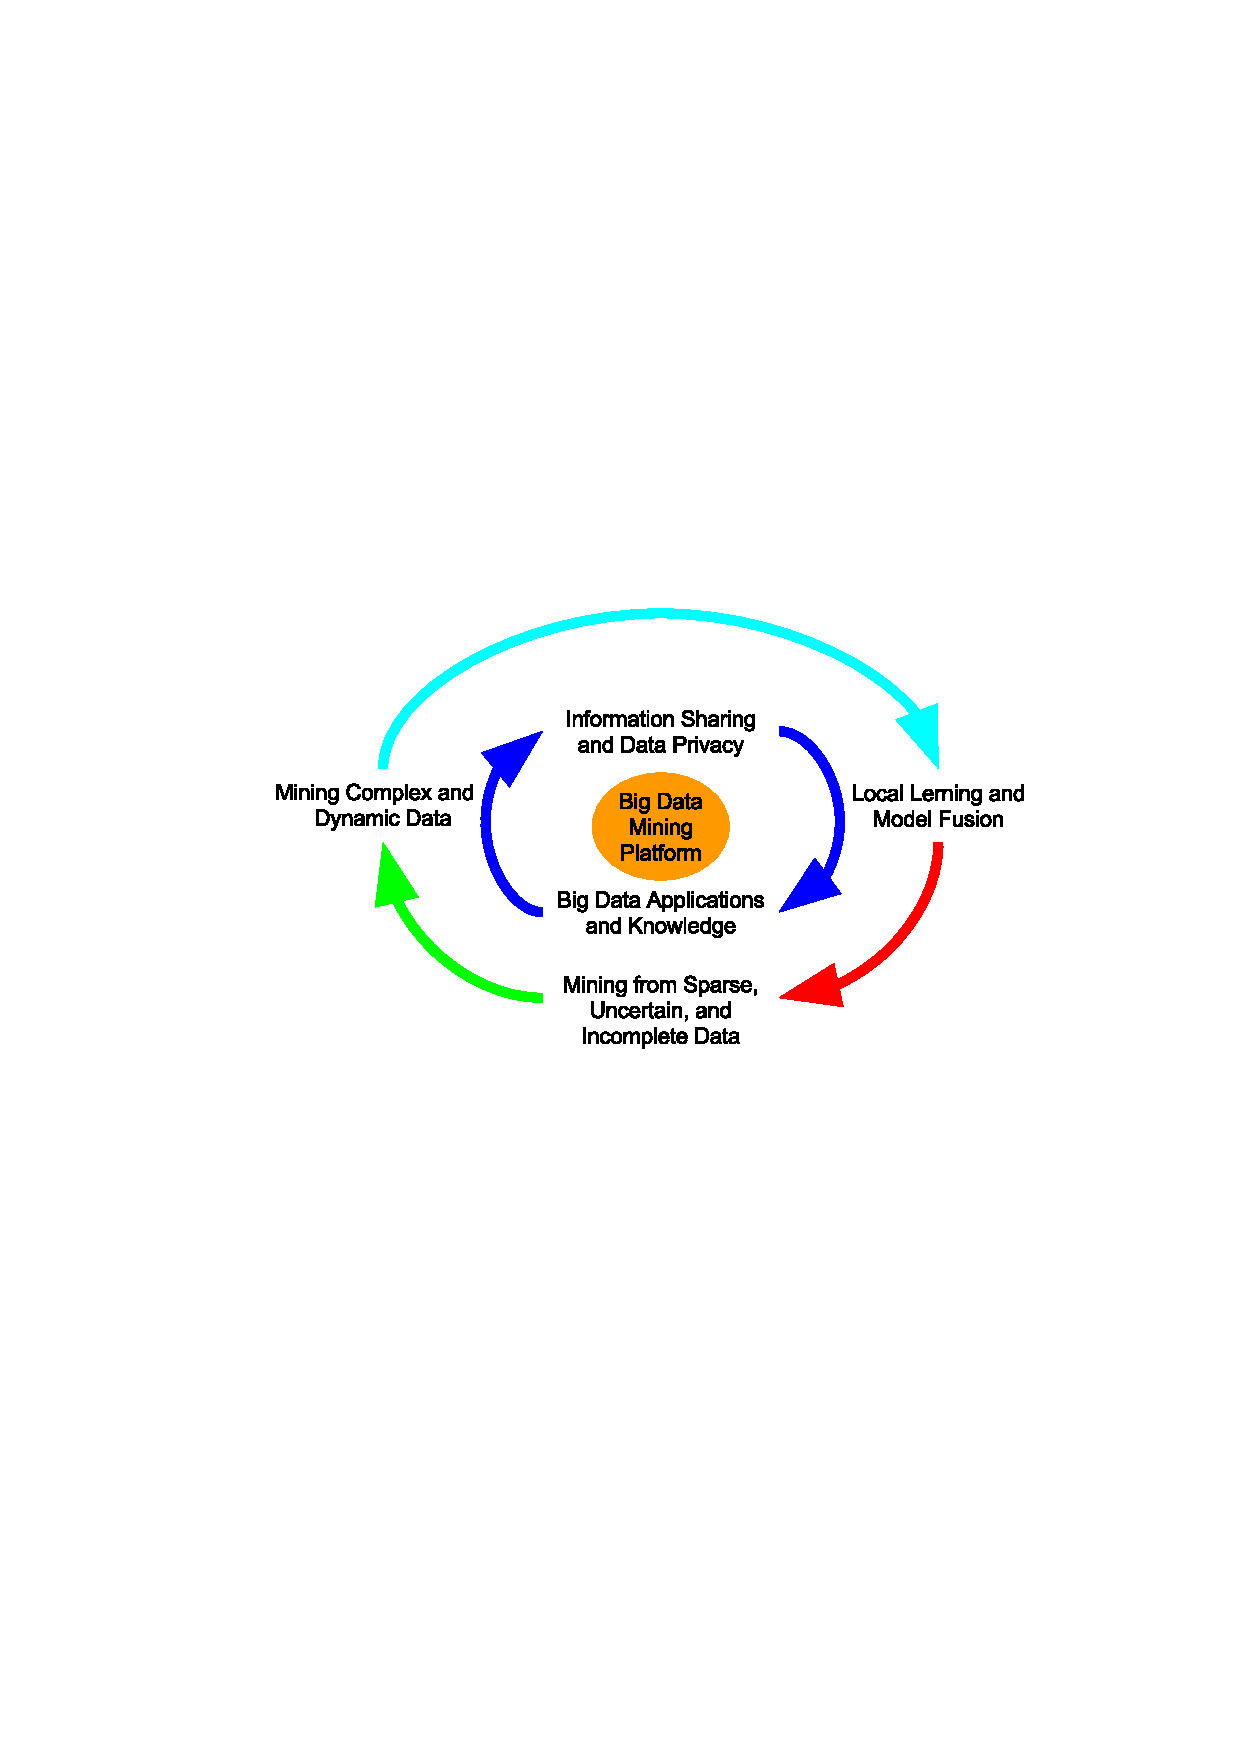
\includegraphics[scale=0.65,trim={120 340 100 280},clip]{img/bigdata42.pdf}
\caption{Datamining mit Big Data \cite{wu2014data}}
\label{bigdata}
\end{figure}
\end{frame}

\section{Fazit~}
\begin{frame}{\insertsectionhead}
\begin{itemize}
\item 
\end{itemize}
\end{frame}

\section*{Diskussion~}
\begin{frame}[highlight]{\insertsectionhead}
\centering
Gibt es Fragen?
\end{frame}

\section*{Danke~}
\begin{frame}{\insertsectionhead}
\centering
Vielen Dank für Ihre Aufmerksamkeit und Ihr Interesse.
\end{frame}

\begin{frame}[allowframebreaks]
\frametitle{Literatur}
%\footnotesize
\bibliographystyle{../IEEEtranBST/IEEEtran} % nummerierung
\setbeamertemplate{bibliography item}{[\theenumiv]}
%\bibliographystyle{apacite}
\bibliography{../lit}
\end{frame}

\end{document}
